% Author: Till Tantau
% Source: The PGF/TikZ manual

\documentclass{article}

\usepackage{pgf}
\usepackage{tikz}
\usetikzlibrary{arrows,automata}
\usepackage[latin1]{inputenc}
\usepackage{verbatim}

\begin{document}

\begin{comment}
:Title: State machine
:Tags: Manual, Automata, Graphs

Another examle from the manual.

| Author: Till Tantau
| Source: The PGF/TikZ manual

\end{comment}

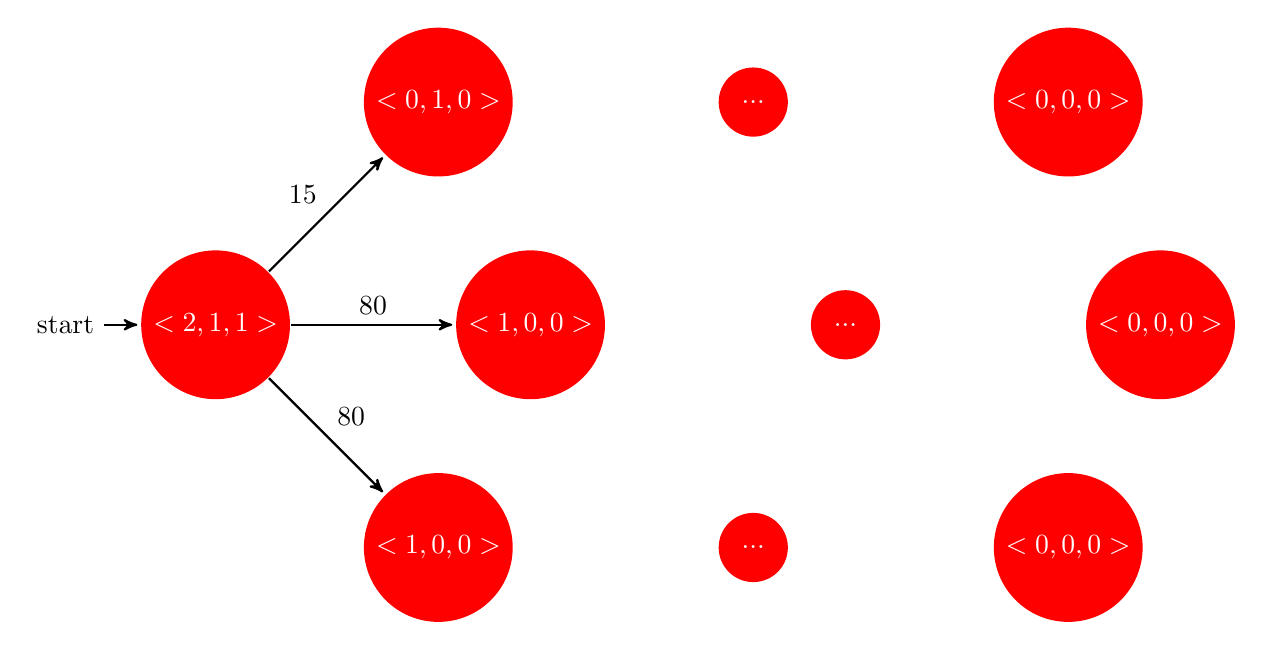
\begin{tikzpicture}[->,>=stealth',shorten >=1pt,auto,node distance=4.0cm,
                    thick]
  \tikzstyle{every state}=[fill=red,draw=none,text=white]

  \node[initial,state] (A)                    {$<2,1,1>$};
  \node[state]         (B) [above right of=A] {$<0,1,0>$};
  \node[state]         (C) [right of=A]       {$<1,0,0>$};
  \node[state]         (D) [below right of=A] {$<1,0,0>$};
  \node[state]         (E) [right of=B]       {$...$};
  \node[state]         (F) [right of=C]       {$...$};
  \node[state]         (G) [right of=D]       {$...$};
  \node[state]         (H) [right of=E]       {$<0,0,0>$};
  \node[state]         (I) [right of=F]       {$<0,0,0>$};
  \node[state]         (J) [right of=G]       {$<0,0,0>$};

  \path (A) edge              node {15} (B)
            edge              node {80} (C)
            edge              node {80} (D)

    
        ;
       
\end{tikzpicture}

\end{document}